\documentclass{report}
\usepackage[utf8x]{inputenc}
\usepackage[a4paper]{geometry}

\usepackage{hyperref}

\usepackage{amsmath,amsthm}

\usepackage{tikz}
\usepackage{verbatim}
\usepackage{simplewick}
\usepackage{enumitem}

%\usepackage[lf]{MinionPro}
\usepackage{newtxtext}
\usepackage{newtxmath}
\usepackage[scr=rsfso,calscaled=.96]{mathalfa}

\usepackage{xfrac}


\usepackage{epic,eepic}
\usepackage{hyperref} \usepackage{bezier} \usepackage{pstricks}
\usepackage{dcolumn}% Align table columns on decimal point
\usepackage{bm}% bold math
%\usepackage{braket}

\newcommand{\One}{\hat{\mathbf{1}}} \newcommand{\eff}{\text{eff}}
\newcommand{\Heff}{\hat{H}_\text{eff}}
\newcommand{\Veff}{\hat{V}_\text{eff}}
\newcommand{\braket}[1]{\langle#1\rangle}
\newcommand{\Span}{\operatorname{sp}}
\newcommand{\tr}{\operatorname{trace}}
\newcommand{\diag}{\operatorname{diag}}
\newcommand{\bra}[1]{\left\langle #1 \right|}
\newcommand{\ket}[1]{\left| #1 \right\rangle} \newcommand{\element}[3]
           {\bra{#1}#2\ket{#3}}

\newcommand{\normord}[1]{ \left\{#1\right\} }

\usepackage{amsmath}


\begin{document}
\section*{Second project fall 2017, FYS-KJM4480/9480}


{\bf All answers must be written out and contain full explanations of
  calculations. \\
Date given: Mon November 6, 2017.\\
Deadline: Mon November 27 at 23:59 PM.}


\subsection*{Introduction}

We present a simple model consisting of an unperturbed
Hamiltonian and a so-called pairing interaction term. It is a model
which to a large extent mimicks some central features of atomic
nuclei, certain atoms and systems which exhibit superfluiditity or
superconductivity.  

In this project, there are no single-particle functions given --- instead, the Hamiltonian is given in terms of its one- and two-body matrix elements and creation and annihilation operators.


We define first the Hamiltonian, with a definition of the model space
and the single-particle basis. Thereafter, we present the various
exercises.

Our model consists of $M$ doubly-degenerate and equally
spaced single-particle levels labelled by $p=1,2,\dots,M$ and spin
$\sigma=\pm$. These states are schematically portrayed in
Fig.~\ref{fig:schematic}, for $M=10$. Each single-particle state is associated with a creation operator $c^\dag_{p\sigma}$. 

We write the Hamiltonian as
\[ \hat{H} = \hat{H}_0 + \hat{V} , \]
where
\[
\hat{H}_0=\sum_{p\sigma}\epsilon_p c_{p\sigma}^{\dagger}c_{p\sigma}, \quad \epsilon_p = \xi\cdot (p-1),
\]
and
\[
\hat{V}=-\frac{1}{2}g\sum_{pq}c^{\dagger}_{p+}
c^{\dagger}_{p-}c_{q-}c_{q+}.
\]
Here, $\hat{H}_0$ is the unperturbed Hamiltonian with a spacing between
successive single-particle states given by $\xi$.

For even number of particles $N$, the ground-state wavefunction of $\hat{H}_0$ is the Slater determinant
\[ \ket{\Phi} = c^\dag_{1+} c^\dag_{1-} \cdots c^\dag_{\sfrac{N}{2}+} c^\dag_{\sfrac{N}{2}-} \ket{-}. \]
This reference wavefunction also defines a Fermi level.


The two-body operator $\hat{V}$ has a very simple form. It represents a \emph{pairing force} and carries a constant strength $g$.  The interaction
can only couple pairs, i.e, it couples two fermions occupying the same level $p$, as indicated by the rightmost four-particle state in
Fig.~\ref{fig:schematic}. There, one of the pairs is excited to the
state with $p=9$ and the other to the state $p=7$. The two middle
possibilities have broken pairs, and will not be present in our treatment. We label
single-particle states below the Fermi level as hole-states with indices $i\sigma$, etc. The
single-particle states above the Fermi level are then particle
states with indices $a\sigma$, etc. 

In our simple model model we have kept both the interaction strength and the
single-particle level spacings as constants, i.e., they are independent of $p$.  In a realistic system like an
atom or the atomic nucleus this is not the case.

It is convenient to define the so-called  \emph{pair creation and pair annihilation operators}
\[
\hat{P}^{\dag}_p \equiv c^\dag_{p+}c^\dag_{p-},
\]
and
\[
\hat{P}_p \equiv c_{p-}c_{p+},
\] 
respectively. We also define the number operator for the level $p$,
\[ \hat{n}_p \equiv \sum_\sigma c^\dag_{p\sigma} c_{p\sigma}. \]
The operator that counts the total number of \emph{pairs} is
\[ \hat{P} = \sum_{p} \hat{P}^\dag_{p}\hat{P}_p. \]
Finally, we define the spin-projection operator
\[
  \hat{S}_z := \frac{1}{2}\sum_{p\sigma} \sigma
  c^\dag_{p\sigma}c_{p\sigma}.
\]

We are now set for the exercises.

\begin{figure*}
\begin{center}
  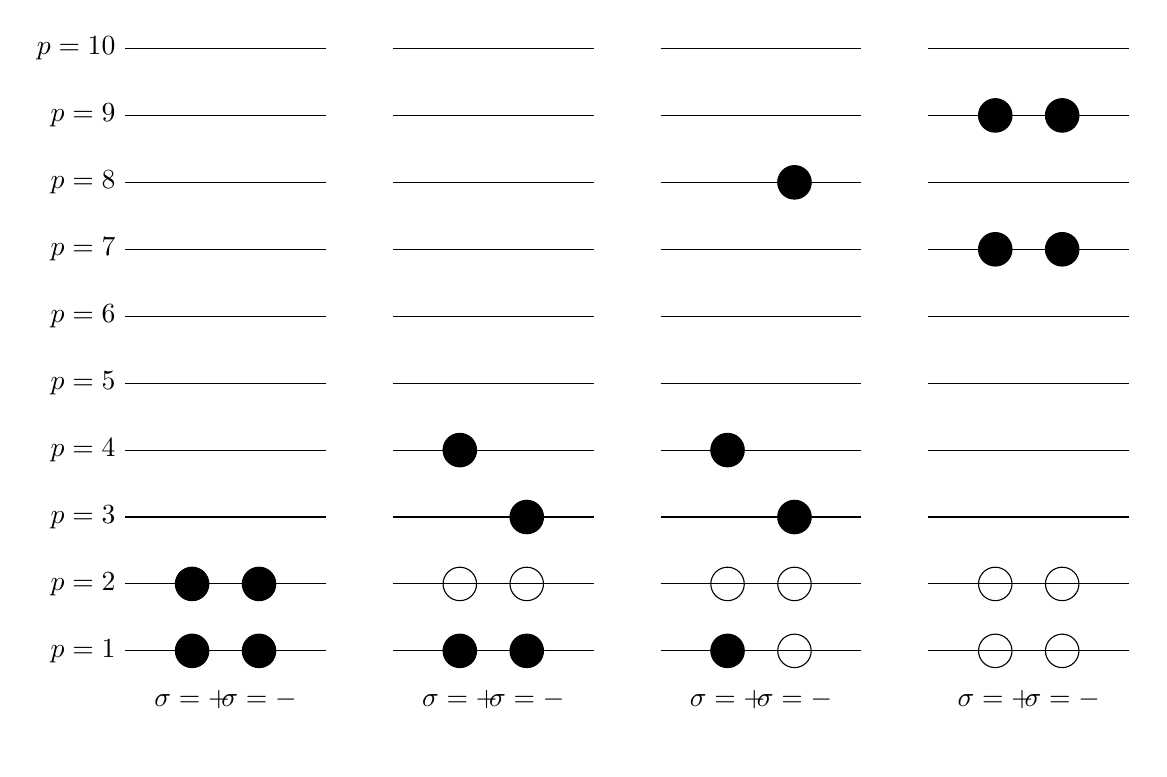
\begin{tikzpicture}[scale=0.85]
    \begin{scope}
      \foreach \i in {1,...,10}
      {
        \draw (-1,\i-1) node[anchor=east] {$p = \i$} --(2,\i-1);
      }
      \filldraw (0,0) node[anchor=north,inner sep=.5cm] {$\sigma=+$} circle (0.25cm); \filldraw (1,0) node[anchor=north,inner sep=.5cm] {$\sigma=-$} circle (0.25cm);
      \filldraw (0,1) circle (0.25cm); \filldraw (1,1) circle (0.25cm);
    \end{scope}
    \begin{scope}[xshift=4cm]
      \foreach \i in {1,...,10}
      {
        \draw (-1,\i-1) --(2,\i-1);
      }
      \filldraw (0,0) node[anchor=north,inner sep=.5cm] {$\sigma=+$} circle (0.25cm); \filldraw (1,0) node[anchor=north,inner sep=.5cm] {$\sigma=-$} circle (0.25cm);
      \draw (0,1) circle (0.25cm); \draw (1,1) circle (0.25cm);
      \filldraw (0,3) circle (0.25cm); \filldraw (1,2) circle (0.25cm);
    \end{scope}
    \begin{scope}[xshift=8cm]
      \foreach \i in {1,...,10}
      {
        \draw (-1,\i-1) --(2,\i-1);
      }
      \filldraw (0,0) node[anchor=north,inner sep=.5cm] {$\sigma=+$} circle (0.25cm); \draw (1,0) node[anchor=north,inner sep=.5cm] {$\sigma=-$} circle (0.25cm);
      \draw (0,1) circle (0.25cm); \draw (1,1) circle (0.25cm);
      \filldraw (0,3) circle (0.25cm); \filldraw (1,2) circle (0.25cm);
      \filldraw (1,7) circle (0.25cm); 
    \end{scope}
    \begin{scope}[xshift=12cm]
      \foreach \i in {1,...,10}
      {
        \draw (-1,\i-1) --(2,\i-1);
      }
      \draw (0,0) node[anchor=north,inner sep=.5cm] {$\sigma=+$} circle (0.25cm); 
      \draw (1,0) node[anchor=north,inner sep=.5cm] {$\sigma=-$} circle (0.25cm);
      \draw (0,1) circle (0.25cm); 
      \draw (1,1) circle (0.25cm);
      \filldraw (0,6) circle (0.25cm); 
      \filldraw (1,6) circle (0.25cm);
      \filldraw (0,8) circle (0.25cm); 
      \filldraw (1,8) circle (0.25cm);
    \end{scope}

  \end{tikzpicture}
\end{center}

\caption{Schematic plot of the possible single-particle levels with
  double degeneracy.  The filled circles indicate occupied particle
  states while the empty circles represent vacant particle (hole)
  states.  The spacing between each level $p$ is constant in this
  picture.  The first two single-particle levels define a reference state $\ket{\Phi}$.  In the second state to the left, one pair is
  broken. This state does not coupled to $\ket{\Phi}$ with our Hamiltonian. The rightmost state has two pairs excited from the reference, and does couple to $\ket{\Phi}$.\label{fig:schematic}}
\end{figure*}

\subsection*{Exercise 1}

\begin{enumerate}[label=\emph{\alph*})]
\item 
  Show that $\hat{H}_0$ and $\hat{V}$ (and therefore also $\hat{H}$)
  commute with $\hat{S}_z$.
\item 
  Show that $\hat{H}_0$ and $\hat{V}$ (and therefore also $\hat{H}$)
  commute with $\hat{P}$.
\item
  Show that $\hat{P}$ commutes with $\hat{S}_z$.
\end{enumerate}

Because of the vanishing commutators above, the Hamiltonian is block diagonal, i.e., we can find a complete set of eigenfunctions $\ket{\Psi_k;S_z,P}$ of $\hat{H}$ such that
\begin{align*}
  \hat{H}\ket{\Psi_k;S_z,P} &= E_{k,S_z,P} \ket{\Psi_k;S_z,P} \\
  \hat{P}\ket{\Psi_k;S_z,P} &= S_z \ket{\Psi_k;S_z,P} \\
  \hat{S}_z\ket{\Psi_k;S_z,P} &= P \ket{\Psi_k;S_z,P}
\end{align*}    

We henceforth focus on the case $N=4$ and $S_z = 0$, $P=2$, and $M=4$ levels. Thus, we seek eigenfunctions $\ket{\Psi_k} \equiv \ket{\Psi_k;0,2}$ and eigenvalues $E_k \equiv E_{k,S_z,P}$. We set $\xi = 1$ in the rest of the project. 


\begin{enumerate}[label=\emph{\alph*})]\setcounter{enumi}{3}
\item
  Show that
  \[ [\hat{P}_p, \hat{P}^\dag_q] = \delta_{pq}(1 - \hat{n}_q). \]
\item
  Show that $\hat{P}\ket{\Phi} = 2\ket{\Phi}$, and that $\hat{S}_z\ket{\Phi} = 0\ket{\Phi}$.
\item
  Explain why the following set of Slater determinants form a basis for the subspace of Hilbert space with $S_z=0$, $P=2$:
  \begin{equation*}
    \ket{p\bar{p}q\bar{q}} \equiv P^\dag_p P^\dag_q \ket{-}, \quad 1 \leq p<q \leq M.
  \end{equation*}
  Here, $\bar{p}$ indicates the state $p-$, while $p$ indicates the state $p+$.
  In a similar manner as in Fig.~1, draw spin-orbital diagrams for $M=4$ and label properly. Draw all the basis states. (See the \LaTeX~source for this document for the code for Fig.~1.) What is the dimension of the subspace (for arbitrary $M$)?
\item
  In a similar manner as Fig.~1, draw spin-orbital diagrams of the basis functions for the subspace $S_z=0$ and $P=0$, $M=4$. (We will not have use for these functions later.) 
\item
Show that you can rewrite the Hamiltonian (with $\xi=1$) as
\[
\hat{H}=\sum_{p}(p-1) \hat{n}_p
-\frac{1}{2}g\left(\sum_{p=1}^4 \hat{P}^\dag_p \right) \left(\sum_{q=1}^4 \hat{P}_q \right).
\]
\end{enumerate}

  We now attack the exact diagonalization (or, full configuration-interaction) of our problem. It can be useful to assign to each basis function $\ket{p\bar{p}q\bar{q}}$ an index $I = 1, 2, \cdots$, where $I=1$ corresponds to $\ket{\Phi}$, and where the doubly excited determinant(s) come next, then the quadruply excited determinant(s). 

\subsection*{Exercise 2}
\begin{enumerate}[label=\emph{\alph*})]
\item
  Show that $\sum_s \hat{P}_s \ket{p\bar{p}q\bar{q}} = \ket{p\bar{p}} + \ket{q\bar{q}}$. Next, compute closed-form expressions of all the matrix elements
  \[ \braket{p'\bar{p}'q'\bar{q'}| \hat{H} |p\bar{p}q\bar{q}}. \]

\item
  We now set $\xi = 1$, and consider $g\in[-1,1]$.
  Using your favorite computing environment, diagonalize the Hamiltonian matrix numerically. Plot the eigenvalues $E_k = E_k(g)$ as function of $g$ in a single figure. Highlight the ground-state energy. Do you observe any degeneracies?

  In a second plot, show the probability $f(g) = |\braket{\Phi|\Psi(g)}|^2/\braket{\Psi|\Psi}$ of finding the 4 particles in the unperturbed ground state.

  Comment the behavior of the ground
  state energy and also of $f(g)$.

\item
   We now turn to the CISD approximation, using $\ket{\Phi}$ as the reference. 
   Explain why the singly excited determinants will not contribute to the exact eigenfunction, i.e., that CISD is the same as CID.

   Show that the doubly excited determinants can be written
   \[ \ket{\Phi_{i\bar{i}}^{a\bar{a}} } \equiv P^\dag_a P_i \ket{\Phi}, \quad i=1,2, \quad a = 3,4. \]
   What is the dimension of the CID space? How many basis functions from the FCI space du you miss?
  
   Find the CID Hamiltonian matrix. Diagonalize this matrix numerically for $g\in[-1,1]$ and plot the \emph{ground-state} eigenvalue as function of $g$. Plot also the ground-state probability. Compare with FCI and discuss.

  (Note that there is no need to introduce Slater--Condon rules, Wick's Theorem, or the rest of the usual CI machinery -- we can simply extract the relevant matrix from the FCI matrix directly.)
\item 
  Next up is Rayleigh--Schrödinger perturbation theory. Write down the expressions for third-order perturbation theory for the ground-state energy for this model. Which matrix elements of $\hat{H}$ are needed?
\item
  Compute the ground-state energy to third order in Rayleigh--Schrödinger perturbation theory, i.e., compute the third order expansion in $g$,
  \[ E_{\text{RSPT3}}(g) = E^{(0)} + g E^{(1)} + g^2 E^{(2)} + g^3 E^{(3)}.\]   
\end{enumerate}

\subsection*{Exercise 3}


The last task is a coupled-cluster treatment, with doubles only, CCD. We will use a doubles operator on the form
\[ \hat{T} = \sum_{ia} t_i^a b^\dag_{a+} b^\dag_{i+} b^\dag_{a-} b^\dag_{i-} = \sum_{ia} t_{i}^a P^\dag_a P_i. \]
It is interesting to note that this resembles a \emph{singles} excitation operator. Note well that the indices $i$ and $a$ refer to each degenerate level -- i.e., they do not depend on spin.

\begin{enumerate}[label=\emph{\alph*})]
\item
  Write down the general CCD wavefunction in terms of $\hat{T}$ and $\ket{\Phi}$ (but do not introduce the amplitudes). Explain why the exponential truncates after second-order terms for our model.
\item
  In a similar manner, write down the general CID wavefunction in intermediate normalization, $\braket{\Phi|\Psi_{\text{CID}}}=1$. Compare with the CCD wavefunction.
\item
  Explain that the CCD energy can be written
  \begin{equation*}
    E_\text{CCD} = \braket{\Phi|\hat{H}(1 + \hat{T})|\Phi}.
  \end{equation*}
  Compute $E_\text{CCD}$ as function of the amplitudes $t_i^a$ in our model, and show that it becomes equal to
  \begin{equation*}
    E_\text{CCD} = 2\epsilon_1+2\epsilon_2 - g - \frac{g}{2}\sum_{ia} t_i^a.
  \end{equation*}
  You can compute this directly, without using generalized Wick's Theorem, etc. The CI matrix element computations should help you. You can of course also use Wick's Theorem.
\end{enumerate}

  We now evaluate the normal-ordered Hamiltonian, in order to find the amplitude equations. The Hamiltonian can be written
  \begin{equation*} 
    \hat{H} = \braket{\Phi|\hat{H}|\Phi} + \underbrace{\hat{F}_N + \hat{V}_N}_{\hat{H}_N}.
  \end{equation*}
  The normal-ordered Fock operator can be written
  \begin{equation}
    \hat{F}_N = \sum_{p\sigma} f_{p} \{ c^\dag_{p\sigma} c_{p\sigma}
    \}, \quad f_{i} = \epsilon_i - \frac{1}{2}g, \quad f_{a} =
    \epsilon_a. \label{eq:fock-n}
  \end{equation}
  Here, we use the notation $\{ \cdots \}$ for the normal-ordering operator, instead of $N(\cdots)$.  The normal-ordered two-body interaction is
  \begin{equation*}
    \hat{V}_N = -\frac{g}{2} \sum_{pq} \{ c^\dag_{p+} c^\dag_{p-} c_{q-} c_{q+}\}. 
  \end{equation*}

\begin{enumerate}[label=\emph{\alph*})]\setcounter{enumi}{3}
\item Show Eqn.~\eqref{eq:fock-n}.
  Explain why the Baker--Campbell--Hausdorff expansion truncates after \emph{two} nested commutators in this case, and explain that the amplitude equations simplify to
  \begin{equation*}
       \braket{\Phi_{i\bar{i}}^{a\bar{a}}|\{\hat{F}_N\hat{T}\}_c|\Phi} +  \braket{\Phi_{i\bar{i}}^{a\bar{a}}|\{\hat{V}_N (1 + \hat{T} + \tfrac{1}{2}\hat{T}^2) \}_c |\Phi } = 0, \quad \forall i,a.
  \end{equation*}
  Explain the $\{\cdots\}_c$ notation.
\item Prove the equations \eqref{ae1}, \eqref{ae2}, \eqref{ae3}, or
  \eqref{ae4} below. You may use the generalized Wick's Theorem for
  products of normal-ordered strings (making sure you take care of the
  $\{\cdots\}_c$ restriction on the contractions). You may also use
  diagrams.\footnote{For Eq.~\eqref{ae4}, it will be convenient to use the
  Kucharski--Bartlett sign scheme. See the book by Bartlett and Shavitt
  (2009), Section 10.3 in particular, where the diagrams of
  Eq.~\eqref{ae4} are treated explicitly. See also Eq.~(9.121) in the same book.}
  \begin{align}
    \braket{\Phi_{i\bar{i}}^{a\bar{a}}|\hat{V}_N|\Phi} &= - \frac{g}{2}, \label{ae1} \\
    \braket{\Phi_{i\bar{i}}^{a\bar{a}}|\{\hat{F}_N\hat{T}\}_c|\Phi} &= 2(f_a - f_i)t_i^a,   \label{ae2} \\
    \braket{\Phi_{i\bar{i}}^{a\bar{a}}|\{\hat{V}_N\hat{T}\}_c|\Phi} &= - \frac{g}{2}\left(\sum_j t_j^a + \sum_b t_i^b\right),\label{ae3} \\
    \frac{1}{2}\braket{\Phi_{i\bar{i}}^{a\bar{a}}|\{\hat{V}_N\hat{T}^2\}_c|\Phi} &= -\frac{g}{2}\left(t_1^3 t_2^4 + t_1^4 t_2^3 - t_i^a \sum_{bj} t_j^b \right)\label{ae4}
%    \frac{1}{2}\braket{\Phi_{i\bar{i}}^{a\bar{a}}|\{\hat{V}_N\hat{T}^2\}_c|\Phi} &= -\frac{g}{2}\left(\sum_j t_j^a \right)\left(\sum_b t_i^b\right)\label{ae4}
%    \frac{1}{2}\braket{\Phi_{i\bar{i}}^{a\bar{a}}|\{\hat{V}_N\hat{T}^2\}_c|\Phi} &= -\frac{g}{2}\left(t_t^3 t_2^4 + t_2^3 t_1^4 \right)\label{ae4}
  \end{align}
\end{enumerate}

  The CCD amplitude equations are
  \begin{equation*}
  0 =    F_i^a(t) \equiv  2(f_a - f_i)t_i^a - \frac{g}{2}\left(1 + \sum_b t_i^b + \sum_j t_j^a + t_1^3 t_2^4 + t_1^4 t_2^3 - t_i^a \sum_{bj} t_j^b \right) 
%  0 =    F_i^a(t) \equiv  2(f_a - f_i)t_i^a - \frac{g}{2}\left(1 + \sum_b t_i^b + \sum_j t_j^a + \sum_b t_i^b \sum_j t_j^a\right) 
  \end{equation*}
  That is, the CCD amplitue equations for our model is written as the zeroes of a polynomial function $F_i^a(t)$, where $t = [t_i^a]$ is a $2\times 2$ matrix (but note the index ranges). We will solve this equation numerically. 

\begin{enumerate}[label=\emph{\alph*})]\setcounter{enumi}{5}
\item
  Show that $F_i^a(t)=0$ is equivalent to 
  \begin{equation}
%     t_i^a = [2(f_i - f_a)] + \sigma]^{-1}\left[\sigma t_i^a - \frac{g}{2}\left(1 + \sum_b t_i^b + \sum_j t_j^a + \sum_b t_i^b \sum_j t_j^a\right)\right].
     t_i^a = [2(f_i - f_a)] + \sigma]^{-1}\left[\sigma t_i^a - \frac{g}{2}\left(1 + \sum_b t_i^b + \sum_j t_j^a + t_1^3 t_2^4 + t_1^4 t_2^3 - t_i^a \sum_{bj} t_j^b\right)\right].
      \label{eq:amp}
  \end{equation}
  Here, $\sigma$ is a shift parameter that will help convergence. We write $t = [t_i^a]$ for the whole matrix of amplitudes.
\item
  Let the right-hand side of Eq.~\eqref{eq:amp} be $\equiv G_i^a(t)$. Define the iteration
  \[ (t^{(k+1)})_i^a = G_i^a(t^{(k)}). \]
  For $g\in [-1,1]$, solve the amplitude equations by iterating this, using $t^{(0)} = 0$ as initial guess. Play around with $\sigma$ until you get convergence for all $g\in[-1,1]$. You will need around 50--100 iterations to reach machine precision. 

\item
  Plot the FCI energy, the CCD energy, and the RSPT energy in one plot and comment your results.
\end{enumerate}



 \end{document}








